\documentclass[tikz]{standalone}
\usepackage{amsmath, amssymb}
\usetikzlibrary{shapes.multipart}

\newcommand{\ii}{\text{i}} % imaginary unit
\newcommand\quot[2]{
    \mathchoice
        {% \displaystyle 
        \text{\raise1ex\hbox{$#1$}\!\Big/\!\lower1ex\hbox{$#2$}}}
        {% \textstyle
            #1\,/\,#2}
        {% \scriptstyle
            #1\,/\,#2}
        {% \scriptscriptstyle  
            #1\,/\,#2}
}% quotient group. Use A/B--->\quot{A}{B}.

\begin{document}
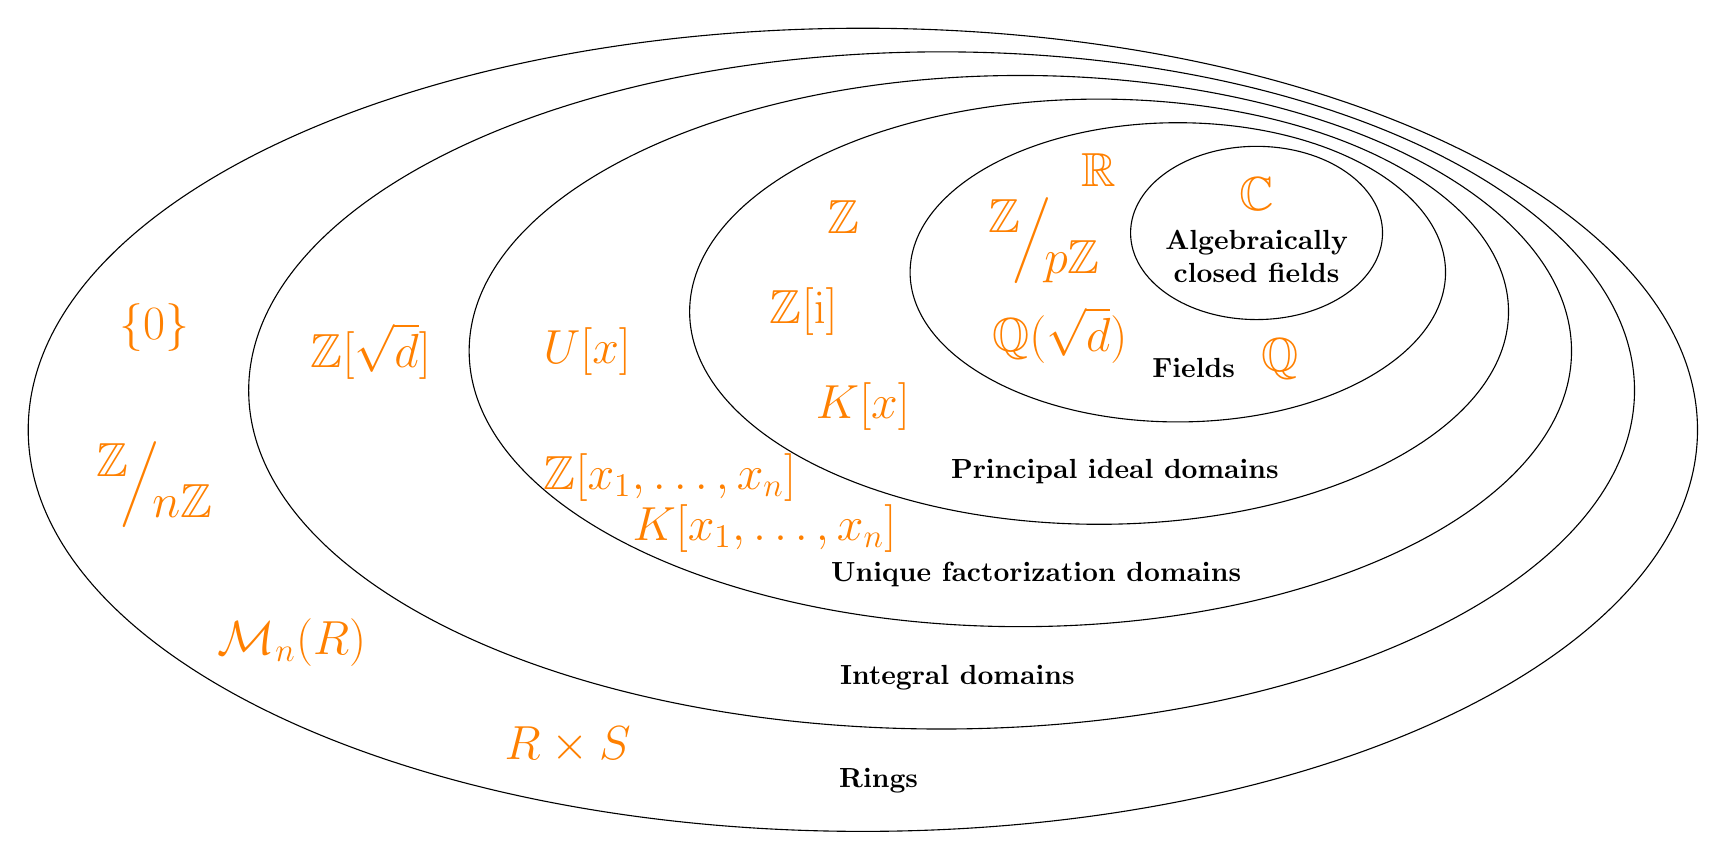
\begin{tikzpicture}
    \node[align=center,font=\bf] at (-1,-0.8) {Algebraically\\closed fields};
    \foreach \X [count=\Y starting from 1.5] in {,Fields,Principal ideal domains,Unique factorization domains,Integral domains,Rings}
    {\draw (-\Y,-\Y/2) ellipse ({1.8*\Y-0.2} and 0.8*\Y+0.3);
    \node[font=\bf] at (-\Y+0.2,-1.31*\Y+0.4) {\X}; }

    \node[color=orange] at (-15,-1.7) {\LARGE $\{0\}$}; %R
    \node[color=orange] at (-15,-3.7) {\LARGE $\displaystyle\quot{\mathbb{Z}}{n\mathbb{Z}}$}; %R
    \node[color=orange] at (-13.25,-5.7) {\LARGE $\mathcal{M}_n(R)$}; %R
    \node[color=orange] at (-9.75,-7) {\LARGE $R\times S$}; %R
    \node[color=orange] at (-12.25,-2) {\LARGE $\mathbb{Z}[\sqrt{d}]$}; %ID. No es DFU en certes condicions (mirar exercici UPC 2.28).
    \node[color=orange] at (-9.5,-2) {\LARGE $U[x]$}; %UFD
    \node[color=orange,rotate=0] at (-8.45,-3.6) {\LARGE $\mathbb{Z}[x_1,\ldots,x_n]$}; %UFD
    \node[color=orange,rotate=0] at (-7.25,-4.25) {\LARGE $K[x_1,\ldots,x_n]$}; %UFD
    \node[color=orange] at (-6.25,-0.3) {\LARGE $\mathbb{Z}$}; %PID
    \node[color=orange] at (-6.75,-1.5) {\LARGE $\mathbb{Z}[\ii]$}; %PID
    \node[color=orange] at (-6,-2.7) {\LARGE $K[x]$}; %PID
    \node[color=orange] at (-3.7,-0.6) {\LARGE $\displaystyle\quot{\mathbb{Z}}{p\mathbb{Z}}$}; %F
    \node[color=orange] at (-3,0.3) {\LARGE $\mathbb{R}$}; %F
    \node[color=orange] at (-0.7,-2.1) {\LARGE $\mathbb{Q}$}; %F
    \node[color=orange] at (-3.5,-1.8) {\LARGE $\mathbb{Q}(\sqrt{d})$}; %F
    \node[color=orange] at (-1,0) {\LARGE $\mathbb{C}$}; %ACF
\end{tikzpicture}
\end{document}